

\documentclass[border=0pt]{standalone}
\usepackage{pgfplots}
\pgfplotsset{width=\linewidth,compat=1.8}
\usepackage{amsmath}
\usepackage{pgfplotstable}
\usepgfplotslibrary{fillbetween}
\providecommand{\datapath}{.}


\pgfplotsset{every tick label/.append style={font=\boldmath\Huge}}
\tikzstyle{every node}=[font=\bfseries\Huge]

\begin{document}
\pgfplotstableread[col sep=comma,]{\datapath/dcfr9_2.csv}\dcfrb
\pgfplotstableread[col sep=comma,]{\datapath/dcfr16_2.csv}\dcfra
\pgfplotstableread[col sep=comma,]{\datapath/cams_2.csv}\cams
 \LARGE
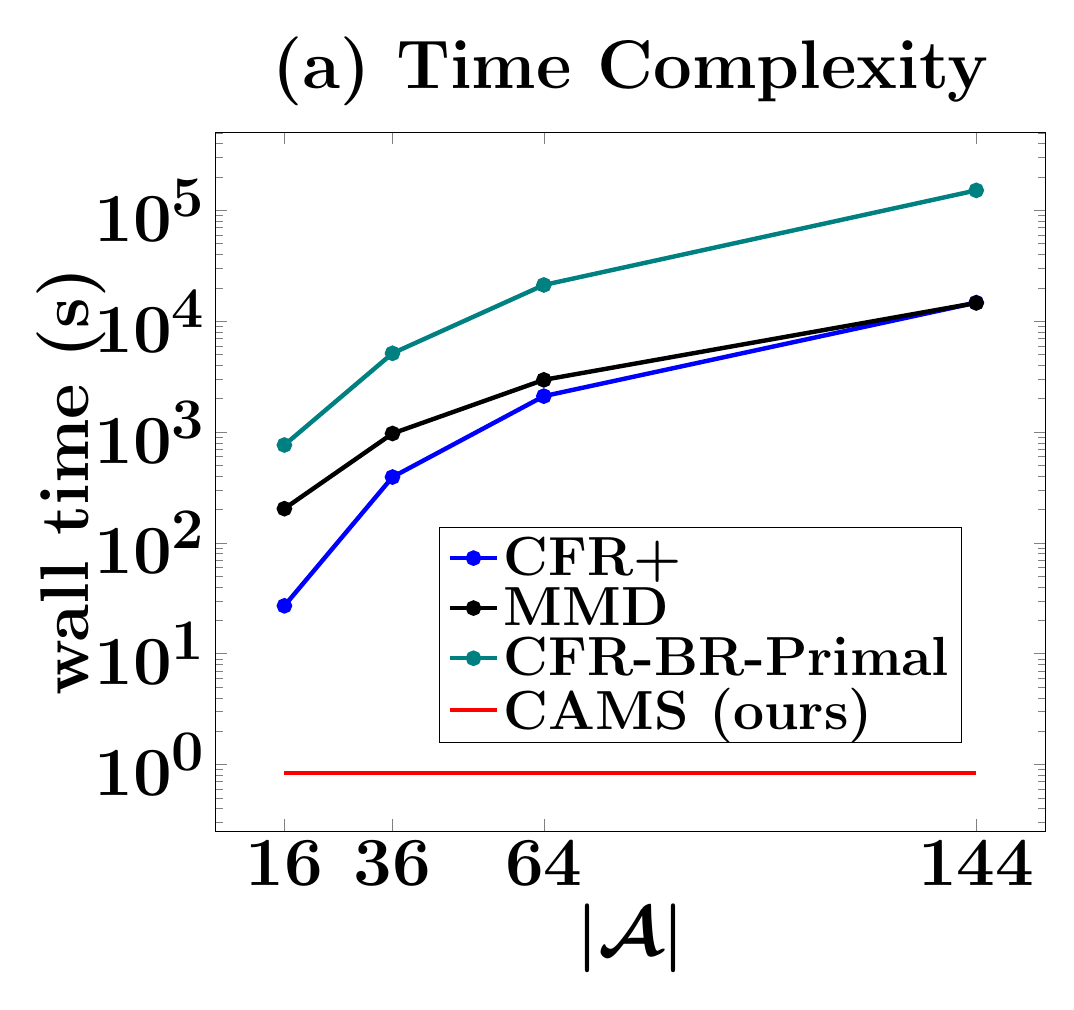
\begin{tikzpicture}[scale=1]
\begin{axis}[title={(a) Time Complexity},
    legend style={nodes={scale=0.8}, style={at={(0.9, 0.435)}}, fill=none},
    legend cell align={left},
    legend entries={CFR+, MMD, CFR-BR-Primal, CAMS (ours)},
    xlabel={$\boldsymbol{|\mathcal{A}|}$},
    ylabel={\textbf{wall time (s)}},
    xtick={16, 36, 64, 144},
    ymode=log,
    % xmode=log,
    ylabel shift=-11pt,
]
% cfr+
\addplot [mark=*, mark size=2pt, ultra thick, blue] coordinates {
(16, 27.05)
(36, 392.77)
(64, 2108.81)
(144, 14707.94)
};
%mmd
\addplot [ultra thick, black, mark=*, mark size=2pt] coordinates {
(16, 203.58)
(36, 970.45)
(64, 2958.36)
(144, 14629.44)
};
%cfr-br-primal
\addplot [ultra thick, teal, mark=*, mark size=2pt] coordinates {
(16, 764)
(36, 5136)
(64, 21238)
(144, 151596)
};
% cams
\addplot [ultra thick, red] coordinates {
(16, 0.842)
(36, 0.842)
(64, 0.842)
(144, 0.842)
};

\end{axis}
\end{tikzpicture}%
% iterations count
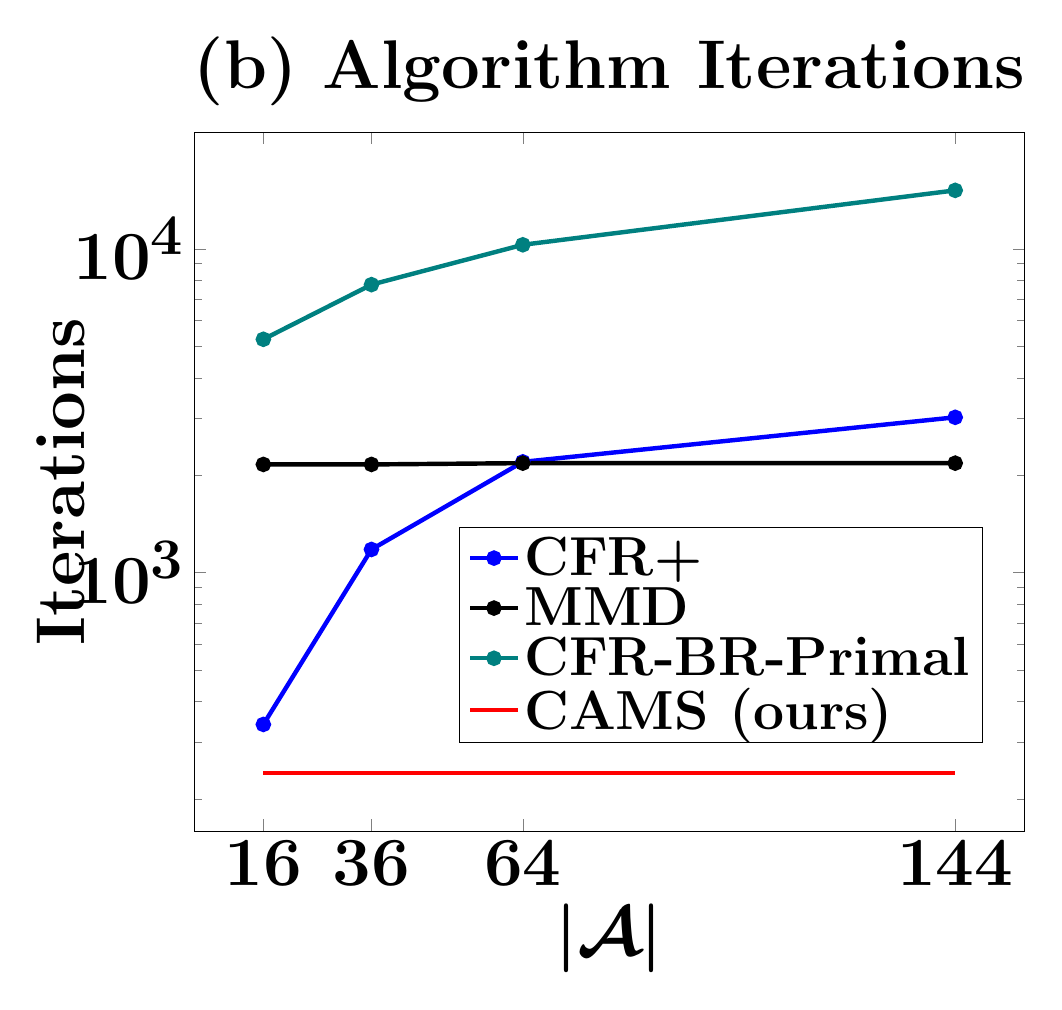
\begin{tikzpicture}[scale=1]
\begin{axis}[title={(b) Algorithm Iterations},
    legend style={nodes={scale=0.8}, style={at={(0.95, 0.435)}}, fill=none},
    legend cell align={left},
    legend entries={CFR+, MMD, CFR-BR-Primal, CAMS (ours)},
    xlabel={$\boldsymbol{|\mathcal{A}|}$},
    ylabel={\textbf{Iterations}},
    xtick={16, 36, 64, 144},
    ymode=log,
    ylabel shift=-11pt,
    % ytick distance=10^.4,
    % log ticks with fixed point,
    % ymin=1e1,
    % ytick={150, 1000, 7000},
    % ytick = {1, 10^1, 10^2, 10^3},
]
% cfr+
\addplot [mark=*, mark size=2pt, ultra thick, blue] coordinates {
(16, 340)
(36, 1180)
(64, 2200)
(144, 3020)
};
%mmd
\addplot [ultra thick, black, mark=*, mark size=2pt] coordinates {
(16, 2160)
(36, 2160)
(64, 2180)
(144, 2180)
};
% cfr-br-primal
\addplot [mark=*, mark size=2pt, ultra thick, teal] coordinates {
(16, 5260)
(36, 7760)
(64, 10300)
(144, 15169)
};
% cams
\addplot [ultra thick, red] coordinates {
(16, 241)
(36, 241)
(64, 241)
(144, 241)
};

\end{axis}
\end{tikzpicture}%
% distance to gt
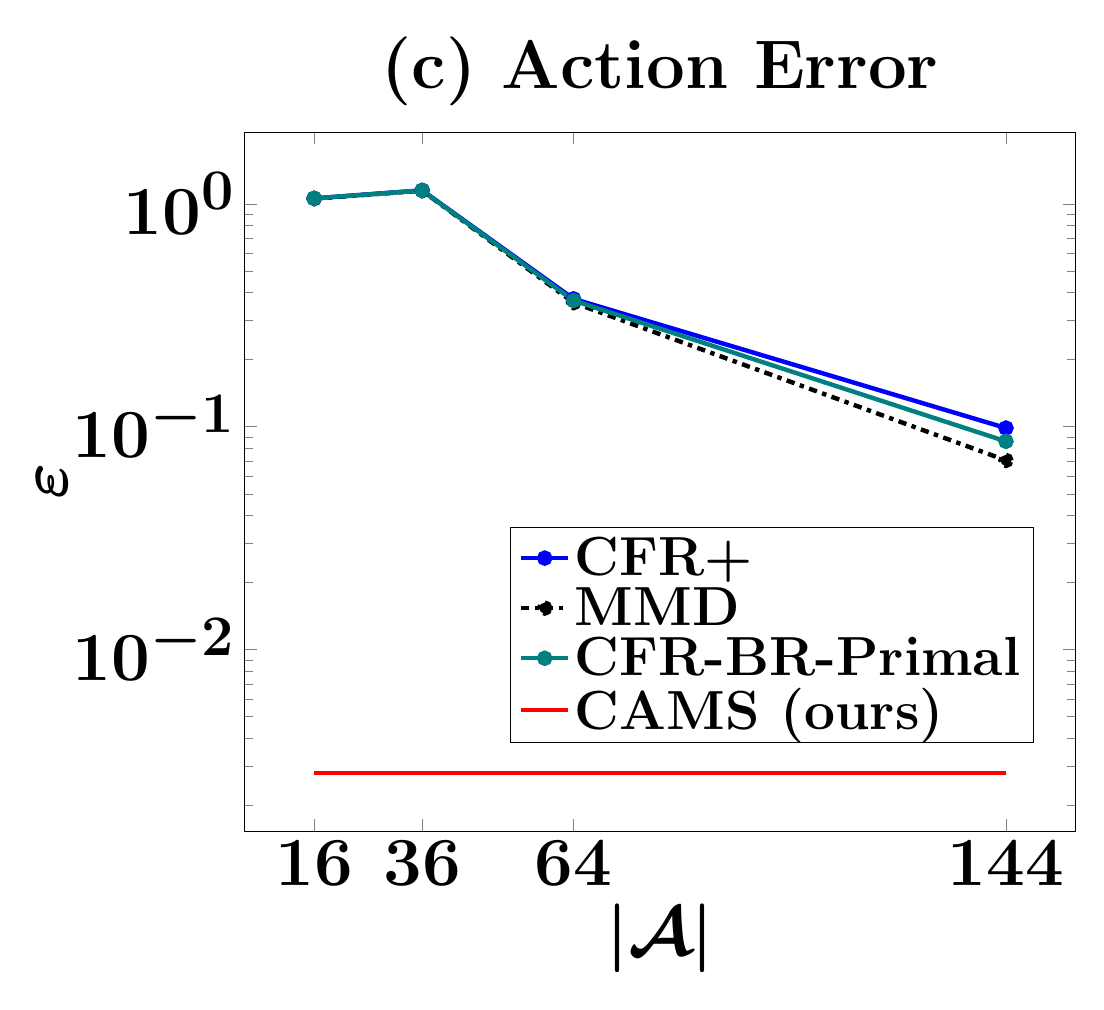
\begin{tikzpicture}[scale=1]
\begin{axis}[title={(c) Action Error},
    legend style={nodes={scale=0.8}, style={at={(0.95, 0.435)}}, fill=none},
    legend cell align={left},
    legend entries={CFR+, MMD, CFR-BR-Primal, CAMS (ours)},
    xlabel={$\boldsymbol{|\mathcal{A}|}$},
    ylabel={$\boldsymbol{\varepsilon}$},
    xtick={16, 36, 64, 144},
    ymode=log,
    ylabel shift=-5pt,
]
% cfr+
\addplot [mark=*, mark size=2pt, ultra thick, blue] coordinates {
(16, 1.0588427800973248)
(36, 1.1494801917079402)
(64, 0.37464195668540257)
(144, 0.09866226893665803)
};
% mmd
% mmd
% [0.5552314866840433,
%  0.5209049957759864,
%  0.5586684894950396,
%  0.6097465051451072]
\addplot[ultra thick, black, mark=*, mark size=2pt, dashdotted] coordinates {
(16, 1.0552507678615948)
(36, 1.146136600348143)
(64, 0.36045590244936615)
(144, 0.07065840307433174)
};
% cfr-br-primal
% 0.6496365514625374,
%  0.2945435474633056,
%  0.1709301707831794,
%  0.03248224069686917
\addplot[ultra thick, mark=*, mark size=2pt, teal] coordinates{
% (16, 0.524)
% (36, 0.568)
% (64, 0.157)
% (144, 0.031)
(16, 1.0581758567678188)
(36, 1.1486716970232314)
(64, 0.3682825954941562)
(144, 0.08599092519673776)
};
% cams
\addplot [ultra thick, red] coordinates {
(16, 0.0028)
(36, 0.0028)
(64, 0.0028)
(144, 0.0028)
};
\end{axis}
\end{tikzpicture}%
\begin{tikzpicture}[scale=1.03]
    \begin{axis}[title={(d) Action Error}, every axis title/.style={above, at={(0.5, 0.986)}},
    legend style={nodes={scale=0.8}, style={at={(0.9, 0.38)}}, fill=none},
    legend cell align={left},
    legend entries={DeepCFR $\boldsymbol{(|\mathcal{A}|=16)}$, DeepCFR $\boldsymbol{(|\mathcal{A}|=9)}$, CAMS (ours)},
    xlabel={$\boldsymbol{t}$},
    ylabel={$\boldsymbol{\bar{\varepsilon}_t}$},
    xtick={0, 0.25, 0.5, 0.75},
    % ytick={0, 5, 10, 15},
    % ymode=log,
    xmax=0.8,
    ylabel shift=-5pt,
]   
% A =16
\addplot [mark=*, mark size=2pt, ultra thick, blue] table[x=x,y=y] {\dcfra};
% A =9
\addplot [mark=*, mark size=2pt, ultra thick, teal] table[x=x,y=y] {\dcfrb};
% cams
\addplot [mark=*, mark size=2pt, ultra thick, red] table[x=x,y=y] {\cams};
% fill betweens
% cfr_9
\addplot [name path=upper,draw=none] table[x=x,y expr=\thisrow{y}+\thisrow{err}] {\dcfrb};
\addplot [name path=lower,draw=none] table[x=x,y expr=\thisrow{y}-\thisrow{err}] {\dcfrb};
\addplot [fill=teal!40, fill opacity=0.4] fill between[of=upper and lower];
% cfr_16
\addplot [name path=upper_2,draw=none] table[x=x,y expr=\thisrow{y}+\thisrow{err}] {\dcfra};
\addplot [name path=lower_2,draw=none] table[x=x,y expr=\thisrow{y}-\thisrow{err}] {\dcfra};
\addplot [fill=blue!40, fill opacity=0.4] fill between[of=upper_2 and lower_2];
% cams
\addplot [name path=upper_3,draw=none] table[x=x,y expr=\thisrow{y}+\thisrow{err}] {\cams};
\addplot [name path=lower_3,draw=none] table[x=x,y expr=\thisrow{y}-\thisrow{err}] {\cams};
\addplot [fill=red!10] fill between[of=upper_3 and lower_3];
    \end{axis}
\end{tikzpicture}
\end{document}



\textbf{Datasets.}
We pre-train on 11 datasets: \textbf{AD-Auditory}~\cite{lahijanian2024auditory}, \textbf{ADFSU}~\cite{vicchietti2023computational}, \textbf{ADSZ}~\cite{pineda2020quantile}, \textbf{APAVA}~\cite{escudero2006analysis}, \textbf{Depression}~\cite{cavanagh2019multiple}, \textbf{PEARL-Neuro}~\cite{dzianok2024pearl}, \textbf{REEG-BACA}~\cite{getzmann2024resting}, \textbf{REEG-PD}~\cite{singh2023evoked}, \textbf{REEG-SRM}~\cite{hatlestad2022bids}, \textbf{TDBrain}~\cite{van2022two}, and \textbf{TUEP}~\cite{veloso2017big}, and fine-tuning on 5 downstream datasets: \textbf{ADFTD}~\cite{miltiadous2023dataset}, \textbf{BrainLat}~\cite{prado2023brainlat}, \textbf{CNBPM}~\cite{amezquita2019novel}, \textbf{Cognision-ERP}~\cite{cecchi2015clinical}, and \textbf{Cognision-rsEEG}. The pre-training datasets include 7 non-AD neurological diseases or healthy subjects and 4 AD datasets, totaling \textit{2,354 subjects and 1,165,361 1-second, 128Hz samples}. All downstream datasets are binary classifications between AD patients and healthy subjects, totaling \textit{615 subjects and 223,039 1-second, 128Hz samples}. The nine AD datasets used for pretraining or fine-tuning consist of \textit{813 subjects} in total. The rationale behind selecting these datasets for pre-training and fine-tuning is discussed in \ref{sub:datasets_selection}. The unified processing pipeline for each dataset is detailed in \ref{sub:data_preprocessing}, with a more detailed description available in Appendix~\ref{sec:datasets_preprocessing}. The statistics for the processed datasets are summarized in Table~\ref{tab:processed_data}.




\textbf{Baselines.}
We compare our method with 10 baselines, including 5 supervised, 3 self-supervised learning, and 2 large EEG foundational models. These selected baselines are state-of-the-art methods or have shown strong performance in EEG or time series classification tasks. The 5 supervised learning methods include \textbf{TCN}~\cite{bai2018empirical}, vanilla \textbf{Transformer}~\cite{vaswani2017attention}, \textbf{Conformer}~\cite{song2022eeg}, \textbf{TimesNet}~\cite{wu2023timesnet}, and \textbf{Medformer}~\cite{wang2024medformer}. The 3 self-supervised learning methods are \textbf{TS2Vec}~\cite{yue2022ts2vec}, \textbf{BIOT}~\cite{yang2024biot}, and \textbf{EEG2Rep}~\cite{mohammadi2024eeg2rep}. The 2 large EEG foundational models are \textbf{LaBraM}~\cite{jiang2024large} and \textbf{EEGPT}~\cite{wangeegpt}. 



\textbf{Implementation.}
All baseline methods and our method's variants, except for LaBraM and EEGPT, are trained under the same code framework. The training epoch for self-supervised pretraining is fixed at 50 epochs, with no early stopping mechanism. The training epoch is set to 100 for fully supervised learning or fine-tuning, with early stopping after 15 epochs of patience based on the best F1 score. The batch sizes for pretraining, fully supervised learning, and fine-tuning are set to 512, 128, and 128, respectively. The optimizer is AdamW. The initial learning rates for pretraining, fully supervised learning, and fine-tuning are set to 0.0002, 0.0001, and 0.0001, respectively, with the CosineAnnealingLR learning scheduler. Gradient norm clipping is set to 4.0, and Stochastic Weight Averaging (SWA)~\cite{izmailov2018averaging} is enabled to benefit inter-subject representation learning. For LaBraM and EEGPT, we use their public code and load their pre-trained model for fine-tuning. We employ four evaluation metrics: sample-level accuracy and F1 score (macro-averaged), and subject-level accuracy and F1 score (macro-averaged) after majority voting, as described in ~\ref{sub:important_setups}. In the self-supervised pre-training stage, all subjects in the datasets are used for training. The ${\lambda_1}$ and ${\lambda_2}$ are both set to 0.5. In the supervised learning or fine-tuning classification stage, the training, validation, and test sets are split based on the subject-independent setup with a ratio of 6:2:2 for each dataset, where each subject appears exclusively in one of these three sets. There is no dataset overlapping between the pre-training and fine-tuning datasets. The training process is conducted with 5 random seeds (41-45) on fixed training, validation, and test sets to compute the mean and standard deviation of the models. All experiments are run on an RTX 4090 GPU and a server with 4 RTX A5000 GPUs, using Python 3.8 and PyTorch 2.0.0 + cu118. Appendix~\ref{sec:implementation_details} provides more details about each method's implementations.
